\documentclass[11pt]{article}

\usepackage{graphicx}
\usepackage{geometry}
\usepackage{tikz-cd}
\usepackage{amsmath}
\usepackage{amssymb}
\usepackage{authblk}
% \usepackage{subfigure}
\usepackage{graphicx}
\usepackage{caption}

\usepackage{listings}
\usepackage{xcolor}

\definecolor{codegreen}{rgb}{0,0.6,0}
\definecolor{codegray}{rgb}{0.5,0.5,0.5}
\definecolor{codepurple}{rgb}{0.58,0,0.82}
\definecolor{backcolour}{rgb}{0.95,0.95,0.92}

\lstdefinestyle{mystyle}{
    backgroundcolor=\color{backcolour},   
    commentstyle=\color{codegreen},
    keywordstyle=\color{magenta},
    numberstyle=\tiny\color{codegray},
    stringstyle=\color{codepurple},
    basicstyle=\ttfamily\footnotesize,
    breakatwhitespace=false,         
    breaklines=true,                 
    captionpos=b,                    
    keepspaces=true,                 
    numbers=left,                    
    numbersep=5pt,                  
    showspaces=false,                
    showstringspaces=false,
    showtabs=false,                  
    tabsize=2
}

\lstset{style=mystyle}



\geometry{a4paper,scale=0.8}
\title{Lab 1: Modeling Packet Losses}
\author{Zhipeng Ye}
\affil{Department of Electrical and Electronic Engineering \\Xi’an Jiaotong-Liverpool University}
\begin{document}

\maketitle
    \section{Hidden Markov Model}
    \paragraph{}
    Gilbert-Elliott Model is packet loss model which is based on two-state Hidden Markov Model.
    In other words, Gilbert-Elliott Model is a simply version of Hidden Markov Model. 
    Therefore, It's necessary to learn more about Hidden Markov Model to understand Gilbert-Elliott Model completely.
    \begin{figure}[ht]
        \centering
        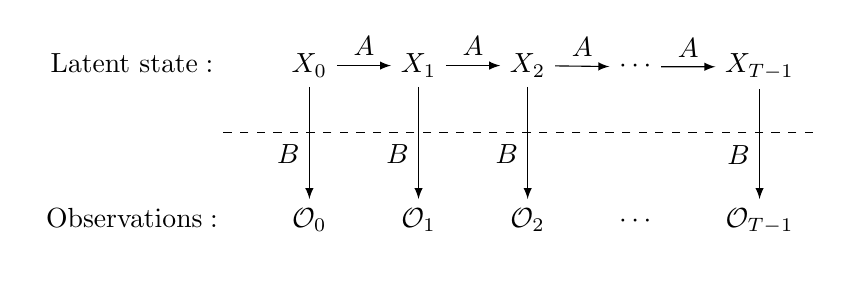
\begin{tikzpicture}
            \matrix[matrix of math nodes,column sep=2em,row sep=4em] (m) {
            \text{Latent state}: &
             X_0 & X_1 & X_2 & \cdots & X_{T-1}\\
            \text{Observations}: & 
             \mathcal{O}_0 & \mathcal{O}_1 & \mathcal{O}_2 & \cdots & \mathcal{O}_{T-1}\\
            };
            \foreach \X in {2,3,4,5}
            {\draw[-latex] (m-1-\X) -- (m-1-\the\numexpr\X+1) node[midway,above]{$A$};
            \ifnum\X=5
            \draw[-latex] (m-1-6) -- (m-2-6) node[pos=0.6,left]{$B$};
            \else
            \draw[-latex] (m-1-\X) -- (m-2-\X) node[pos=0.6,left]{$B$};
            \fi}
            \draw[dashed] ([yshift=1ex]m.east) -- ([yshift=1ex]m.east-|m-1-1.east);
            \end{tikzpicture}
        \caption{Hidden Markov Model}
        \label{fig:ch5:jointentropy}
    \end{figure}
    \paragraph{}
    Hidden Markov Model introduce two random variable - Latent state and Observations. Latent state is a variable that we can't see.
    Observations is a variable that we can observe at the experiment.
    Furtheremore, HMM also has three parameters - initial probability vector $\pi$, transition probability matrix $A$,
    emission probability matrix $B$. So if we can compute three parameters $\{A,B,\pi\}$, we will reconstruct HMM.
    Researchers have developed numerous approaches to estimate parameters of Hidden Markov Model (HMM) such as Forward/Backward Algorithm.
    \paragraph{}
    Markov Model simplifies the Hidden Markov Model (HMM). It only uses two parameters $\{A,\pi\}$ and removes the Latent state. Maximum likelihood estimation (MLE) is a good way to 
    estimate these parameters. The relationship between Hidden Markov Model and Markov Model is similar to the relation between Gilbert-Elliott Model (GM) and Simple Gilbert-Elliott Model (SGM). Section two of this article will demonstrate the reason. 
    \section{Gilbert-Elliott Model}
    \paragraph{}Gilbert-Elliott Model resembles Hidden Markov Model. To be specific, Gilbert-Elliott Model has two state - $\{Good, Bad\}$ , transition matrix $\boldsymbol{P}=\left[\begin{array}{cc}(1-p) & q \\ p & (1-q)\end{array}\right]$ and emission probability vector $\left[\begin{array}{cc}1-k&1-h\end{array}\right]^T$.
    \paragraph{}
        \begin{figure}[ht]
        \centering
        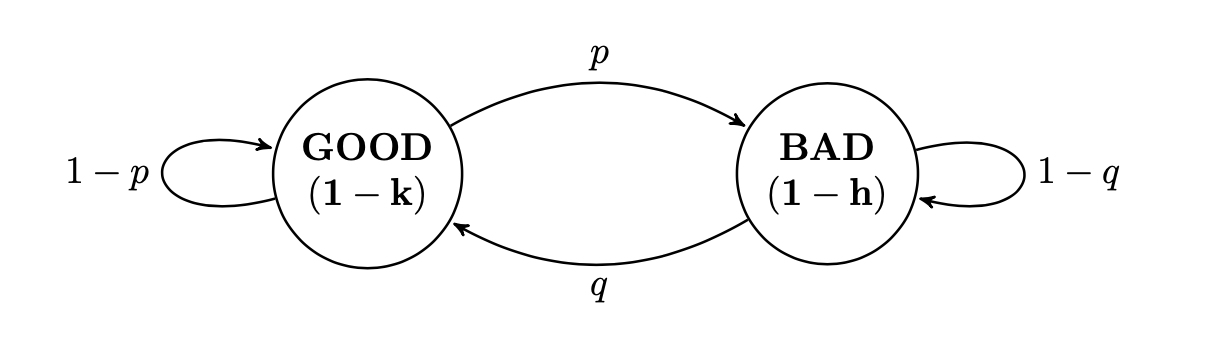
\includegraphics[scale=0.5]{figure1.png}
        \caption{Gilbert-Elliott Model}
        \label{fig:label}
    \end{figure}
    Furtheremore, we can obtain the other parameters of Gilbert-Elliott Model such as the steady state probability vector $\pi$, packet loss probability $p_L$ and the probability distribution of loss run length $p_k$.
    The steady state probability vector $\boldsymbol \pi$ satisfies the following conditions:
    \begin{equation}
        \boldsymbol{\pi} = \boldsymbol{P}\boldsymbol{\pi}, \boldsymbol{1}^T\boldsymbol{\pi}
    \end{equation}
    where 
    \begin{equation}
        \boldsymbol{\pi} = \left[
        \begin{array}{c}
            \pi_{G} \\ \pi_{B}
        \end{array}        
        \right]
    \end{equation}
    The steady state probabilities exist for $0<p$, $q<1$ and are given by 
    \begin{equation}
        \pi_G = \frac{q}{p+q},\pi_B = \frac{p}{p+q}
    \end{equation}
    From equation (3), we can get packet loss probability $p_L$ as follows:
    \begin{equation}
        p_L = (1-k)\pi_G + (1-h)\pi_B
    \end{equation}
    The special cases of $k=1$ and $k=1,h=0$ are called a Gilbert Model (GM) and a simple Gilbert Model
(SGM), respectively.
Note that in case of the SGM, the probability distribution of loss run length has a geometric distribution,
i.e.,
\begin{equation}
    p_{k} \triangleq \text { Prob }\{\text { loss run length }=k\}=q(1-q)^{k-1} \text { for } k=1,2, \ldots, \infty
\end{equation}
\section{Estimation of parameters}
\subsection{Simple Gilbert Model (SGM)}
\paragraph{}
Because $0,1$ represent $\{Good,Bad\}$ respectively. The probabilities from \emph{Good to Bad} is equal to $P(1|0)$ and 
the probabilities from \emph{Bad to Good} is equal to $P(0|1)$. According to \emph{Bayes theorem}, 
\begin{equation}
    \begin{array}{lr}
    p = P(1|0) = \frac{P(01)}{P(0)} = \frac{n_{01}}{n_0} &\\ \\
    q = P(0|1) = \frac{P(10)}{P(1)} = \frac{n_{10}}{n_1}
    \end{array}
\end{equation}
$n_{10}$ means the times 0 follows 1 . $n_{01}$ means the times 1 follows 0. $n_0$ represents the times of 0. $n_1$ represents the times of 1.
\subsection{Gilbert Model (GM)}
Gilbert applied a method to decide the parameters of GM \cite{Gilbert Model}.
Firstly, the parameters of ${p,q,h}$ can be estimated from another parameters of ${a,b,c}$. 
The expression equation of ${a,b,c}$ is as follow:
\begin{equation}\label{abc}
    a=P(1), b=P(1 | 1), c=\frac{P(111)}{P(101)+P(111)}
\end{equation}
Finally, we can get parameters of Gilbert Model by the following relation between these variables.
\begin{equation}\label{pqh}
    1-q=\frac{a c-b^{2}}{2 a c-b(a+c)}, h=1-\frac{b}{1-q}, p=\frac{a q}{1-h-a}
\end{equation}

\section{Experiment Task}
In this experiment, we simulate the Simple Gilbert Model (SGM) and Gilbert Model (GM) separately.
\subsection{Simple Gilbert Model (SGM)}
\subsubsection{Construct model}
The script and detailed comments for Constructing Simple Gilbert Model is attached at the appendix \ref{CSGM}.
The main implement is here.
\begin{verbatim}
# main loop
for i in range(len):
    # if the random sequence is large than the transition probability
    # we must change the state for example 0 -> 1 or 1 -> 0
    if statechange[i] > tr[state, state]:
        # transition into the other state
        state ^= 1
    # add a binary value to output
    seq[i] = state
\end{verbatim}
As we can see from the code segment, if the sequence[i] is large than the transition probability, the start will flip from $0$ to $1$ or from $1$ to $0$.
\subsubsection{Estimate model parameters}
To determine the parameters of $p,q$, I write the script which is in Appendix \ref{ESGM} to count the number of times where binary sequence occurs.
Consequently, I observe the value of $p,q$ is 
\begin{equation}
    \begin{array}{lr}
    p = 0.14727215389467044 & \\
    q = 0.2550574084199016
    \end{array}
\end{equation}
The steady vector $\boldsymbol{\pi}$:
\begin{equation}
    \pi_G = \frac{q}{p+q} = 0.6339514475460747, \pi_B = \frac{p}{p+q} = 0.3660485524539253
\end{equation}
Packet loss probability $p_L$ as follows:
\begin{equation}
    p_L = \pi_B = 0.3660485524539253
\end{equation}
The probability distribution of loss run length has a geometric distribution:
\begin{equation}
    p_{k} =0.2550574084199016(0.7449425915800985)^{k-1} \text { for } k=1,2, \ldots, \infty \label{distributionofSGM}
\end{equation}
\subsubsection{Comparison and discussion}
Based on the parameters we observed, I run the SGM script to generate the sequence which has the same length as the supplied sequence.
Here is the shell command:
\begin{verbatim}
    python sgm_generate.py -L 10000 -T 0.8527278461053296,0.2550574084199016,
    0.14727215389467044,0.7449425915800985
\end{verbatim}
Next, I compare the histogram and power spectrum density between given data and generated data. The plot script can be seen in the appendix \ref{PLTSGM}.
\begin{figure}[htbp]
    \centering
    \begin{minipage}[t]{0.48\textwidth}
    \centering
    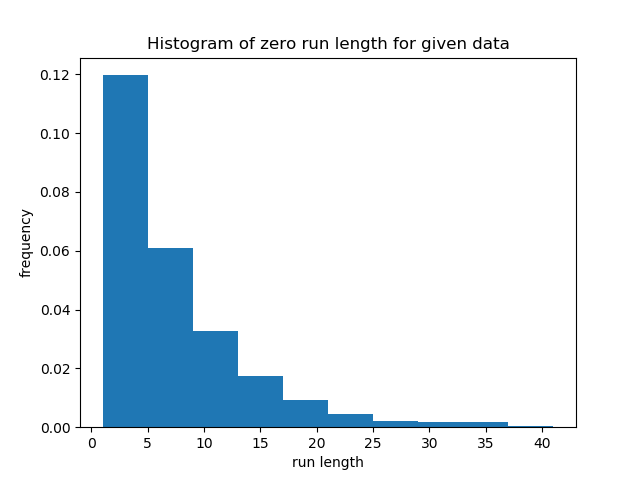
\includegraphics[width=6cm]{Histogram_of_zero_run_length_for_given_data.png}
    \caption{SGM zero length for given data}
    \end{minipage}
    \begin{minipage}[t]{0.48\textwidth}
    \centering
    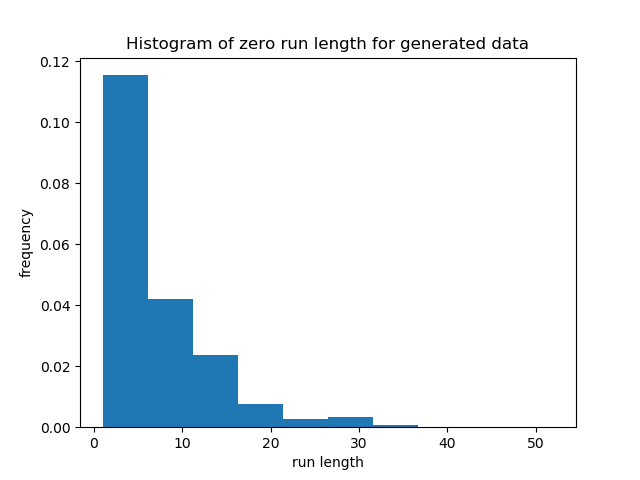
\includegraphics[width=6cm]{Histogram_of_zero_run_length_for_generated_data.png}
    \caption{SGM zero length for generated data}
    \end{minipage}
\end{figure}
\begin{figure}[htbp]
    \centering
    \begin{minipage}[t]{0.48\textwidth}
    \centering
    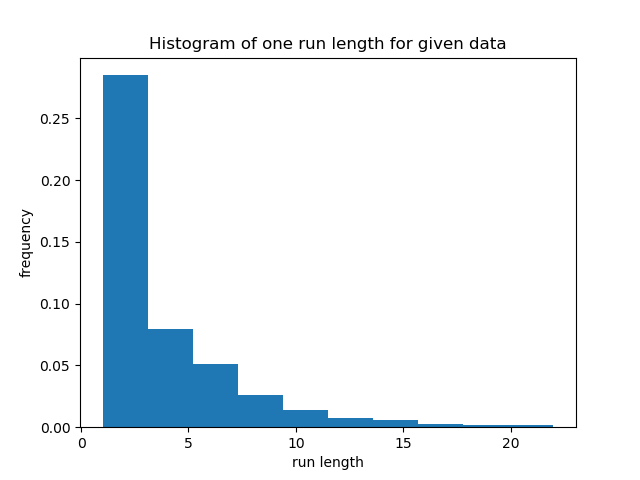
\includegraphics[width=6cm]{Histogram_of_one_run_length_for_given_data.png}
    \caption{SGM one length for given data}
    \end{minipage}
    \begin{minipage}[t]{0.48\textwidth}
    \centering
    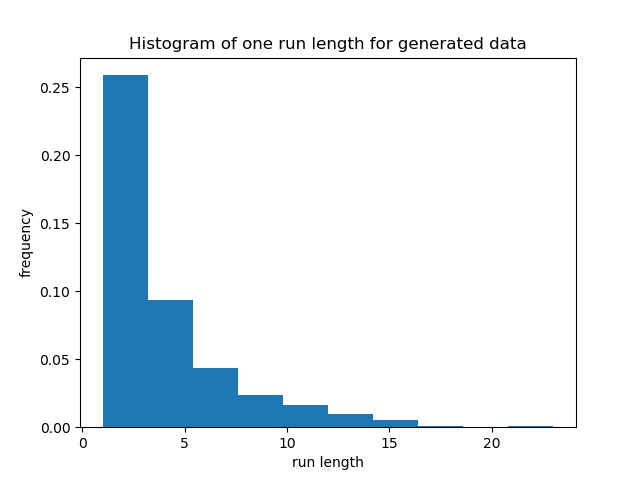
\includegraphics[width=6cm]{Histogram_of_one_run_length_for_generated_data.png}
    \caption{SGM one length for generated data}
    \end{minipage}
\end{figure}
As we can see from the pictures, the given data is similar to the generated data, because random variable \textbf{\emph{submit the same stochastic process}}. 
Interestingly, the whole process of parameters estimation \textbf{is similar to the learning process in Machine learning} and Hidden Markov Model is a significant model of Machine learning.
In addition, we have known the distribution of loss run length from equation \ref{distributionofSGM}. 
Therefore we can generate theoretical curve. 
\begin{figure}[htb]
    \centering
    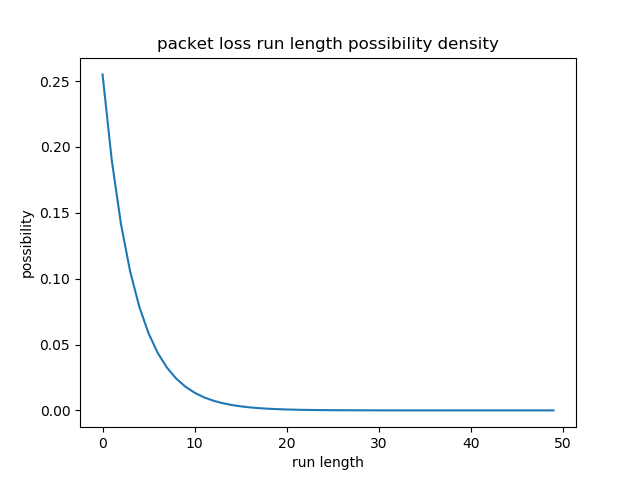
\includegraphics[scale = 0.6]{packet_loss_run_length_possibility_density.png}
    \caption{SGM packet loss run length theoretical possibility density}
    \label{SGMTD}
\end{figure}
\textbf{From figure \ref{SGMTD}}, we can learn that the one length histogram submit to the theoretical cure.
The script for generate theoretical curve is attached at appendix \ref{TSPLC}.
\paragraph{}
Furtheremore, I compare the power spectrum density PSD for given sequence and generated sequence.
we can see from \textbf{Figure 8} and \textbf{Figure 9}, they have similar distribution.
In general, the estimated parameters is correct.
\begin{figure}[htbp]
    \centering
    \begin{minipage}[t]{0.48\textwidth}
    \centering
    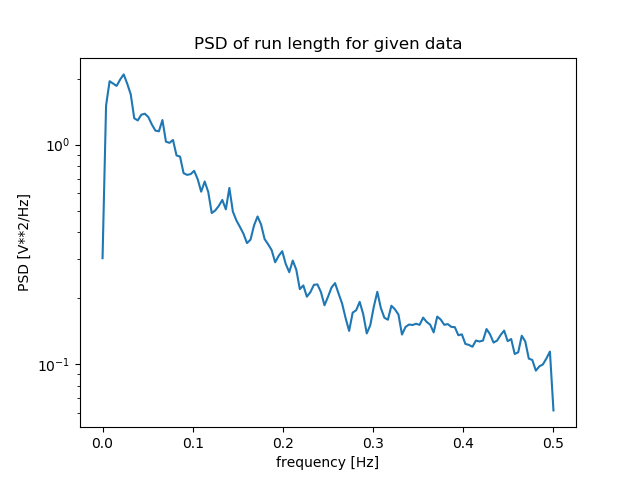
\includegraphics[width=6cm]{PSD_of_run_length_for_given_data.png}
    \caption{SGM PSD of given data}
    \end{minipage}
    \begin{minipage}[t]{0.48\textwidth}
    \centering
    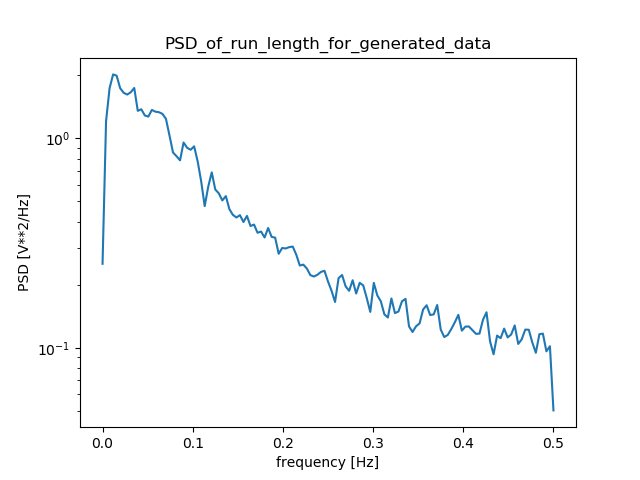
\includegraphics[width=6cm]{PSD_of_run_length_for_generated_data.png}
    \caption{SGM PSD of generated data}
    \end{minipage}
\end{figure}
\clearpage
\subsection{Gilbert Model (GM)}
Gilbert Model has one more parameters $H$ than Simple Gilbert Model (SGM). Therefore following steps must be around parameter $H$.
\subsubsection{Construct model}
The script and detailed comments for Constructing Gilbert Model is attached at the appendix \ref{CGM}.  The main implement is here:
\begin{lstlisting}[language=Python]
    for i in range(len):
    # if the random sequence is large than the transition probability
    # we must change the state for example 0 -> 1 or 1 -> 0
    if statechange[i] > tr[state, state]:
        # transition into the other state
        state ^= 1
    # if latent state is 1 (Bad state), we must consider the emission probability to
    # generate sequence
    if state == 1:
        randomvalue = random.random()
        if randomvalue <= emission_probability:
            loss_state = 1

    # add a binary value to output
    seq[i] = loss_state

    loss_state = 0
\end{lstlisting}
To create Gilbert Model, I introduce loss state to consider emission probability. if the random value is large than $1-H$, the Bad state will cause packet loss.
\subsubsection{Estimate model parameters}
To determine the parameters of $a,b,c$ and $p,q,h$, I write the script to estimated them at appendix \ref{EGM}.
According to equation \ref{abc} and \ref{pqh}, we can get these parameters of Gilbert Model.
Finally, I obtain the parameters of Gilbert Model.
\begin{equation}
    \begin{array}{lr}
        a=0.3658,
        b=0.7446692181519955,
        c=0.9301369863013699\\
        p=0.1449793136870664,
        q=0.2469390489546801,
        h=0.01114349759030242
    \end{array}
\end{equation}
The steady vector $\boldsymbol{\pi}$:
\begin{equation}
    \pi_G = \frac{q}{p+q} = 0.6300777725498095, \pi_B = \frac{p}{p+q} = 0.36992222745019054
\end{equation}
Packet loss probability $p_L$ as follows:
\begin{equation}
    p_L = (1-h)\pi_B = 0.3658
\end{equation}
The probability distribution of loss run length has a geometric distribution:
\begin{equation}
    \begin{array}{lr}
        p_{k} =(1-q)^{k-1}(1-h)^{k-1}[1-(1-q)(1-h)] 
        \\=0.7530609510453199 ^{k-1}*0.9888565024096976^{k-1}*0.2553307818480045
        \\= 0.2553307818480045 * 0.7446692181519955^{k-1}
        \text { for } k=1,2, \ldots, \infty \label{distributionofSGM}
    \end{array}
\end{equation}
\subsubsection{Comparison and discussion}
Based on the parameters we observed, I run the SGM script to generate the sequence which has the same length as the supplied sequence.
Here is the shell command:
\begin{verbatim}
    python gm_generate.py -L 10000 -T 0.8550206863129336,0.2469390489546801,
    0.1449793136870664,0.7530609510453199 -H 0.01114349759030242
\end{verbatim}
Next, I compare the histogram and power spectrum density between given data and generated data. The plot script can be seen in the appendix \ref{PLTGM}.
As we can see from the Figure 10 - 13, the given data is \textbf{similar} to the generated data. 
Furtheremore, GM has a \textbf{better performance to simulate the given data than SGM}, when we compare GM histogram and SGM histogram.
In my opinion, Maybe GM has one more parameters $H$ which can improve the performance of model.
\textbf{This concept can be easily seen in Machine learning and Deep learning}. To some extent, \emph{the more parameters we consider in the model, the better the model fit the training set}.
\begin{figure}[htbp]
    \centering
    \begin{minipage}[t]{0.48\textwidth}
    \centering
    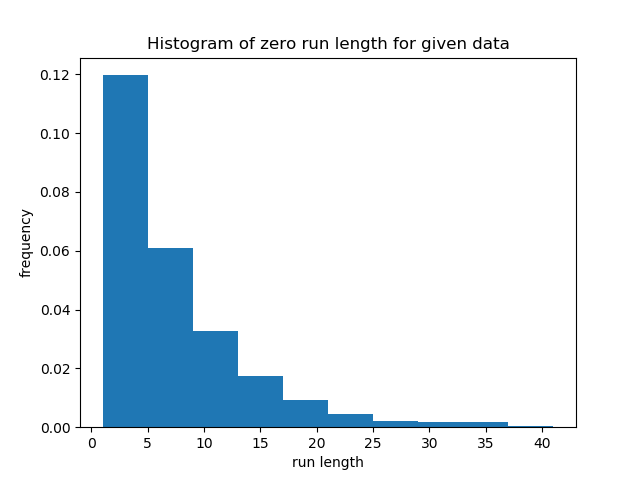
\includegraphics[width=6cm]{GM_Histogram_of_zero_run_length_for_given_data.png}
    \caption{GM zero length for given data}
    \end{minipage}
    \begin{minipage}[t]{0.48\textwidth}
    \centering
    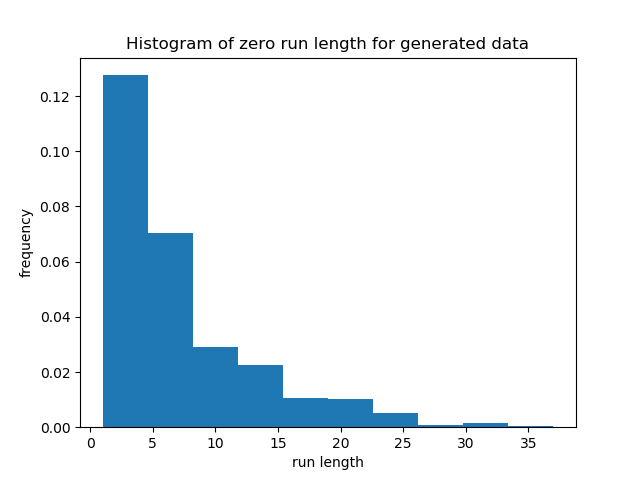
\includegraphics[width=6cm]{GM_Histogram_of_zero_run_length_for_generated_data.png}
    \caption{GM zero length for generated data}
    \end{minipage}
\end{figure}
\begin{figure}[htbp]
    \centering
    \begin{minipage}[t]{0.48\textwidth}
    \centering
    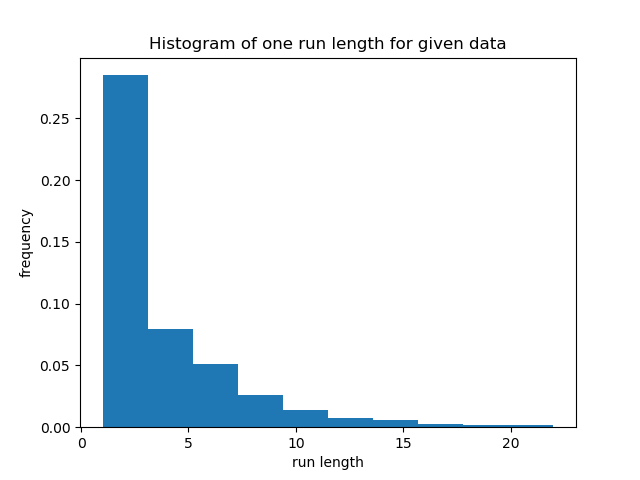
\includegraphics[width=6cm]{GM_Histogram_of_one_run_length_for_given_data.png}
    \caption{GM one length for given data}
    \end{minipage}
    \begin{minipage}[t]{0.48\textwidth}
    \centering
    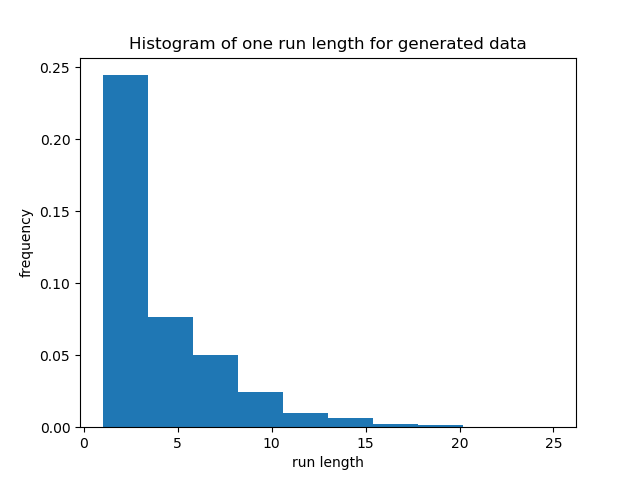
\includegraphics[width=6cm]{GM_Histogram_of_one_run_length_for_generated_data.png}
    \caption{GM one length for generated data}
    \end{minipage}
\end{figure}
Furtheremore, based on the theoretical packet loss distribution, I write script to plot the theoretical curve.
The  script  for  generate  theoreticalcurve is attached at appendix \ref{TPLC}.
\begin{figure}[htb]
    \centering
    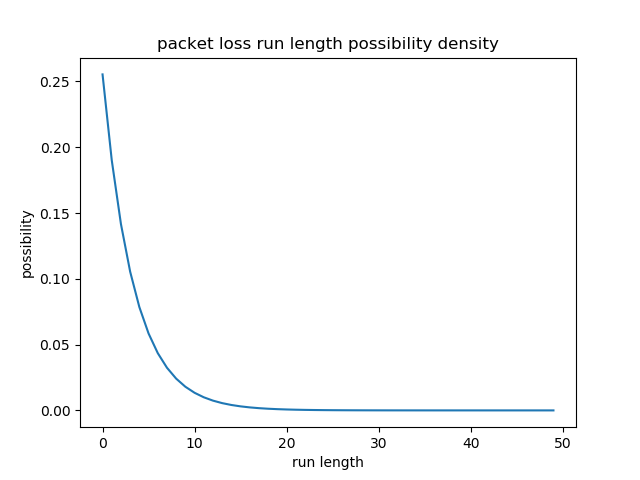
\includegraphics[scale = 0.6]{GM_packet_loss_run_length_possibility_density.png}
    \caption{SGM packet loss run length theoretical possibility density}
    \label{GMTD}
\end{figure}
\textbf{From figure \ref{GMTD}}, we can learn that the one length histogram submit to the theoretical cure.
\paragraph{}
Furtheremore, I compare the power spectrum density PSD for given sequence and generated sequence.
we can see from \textbf{Figure 15} and \textbf{Figure 16}, they have similar distribution.
In general, the estimated parameters is correct.
\begin{figure}[htbp]
    \centering
    \begin{minipage}[t]{0.48\textwidth}
    \centering
    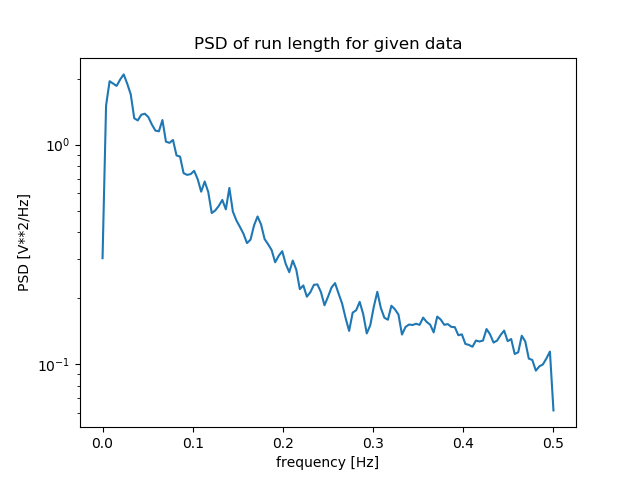
\includegraphics[width=6cm]{GM_PSD_of_run_length_for_given_data.png}
    \caption{GM PSD of given data}
    \end{minipage}
    \begin{minipage}[t]{0.48\textwidth}
    \centering
    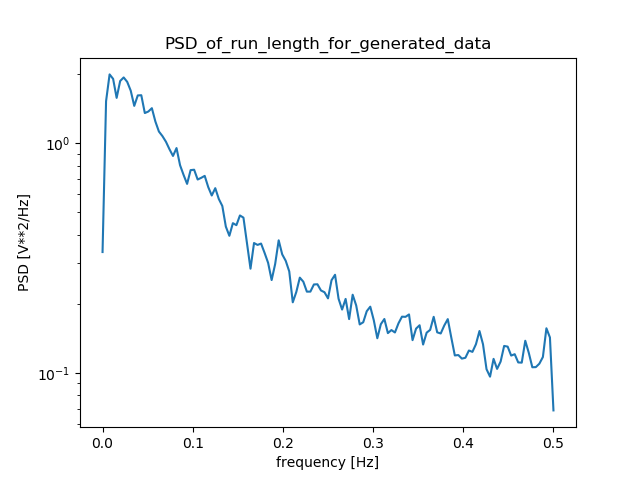
\includegraphics[width=6cm]{GM_PSD_of_run_length_for_generated_data.png}
    \caption{GM PSD of generated data}
    \end{minipage}
\end{figure}
\clearpage
\appendix{\textbf{Detailed Python Script Appendix}}
\section{Construct Simple Gilbert Model (SGM)} \label{CSGM}
\begin{lstlisting}[language=Python]
#!/usr/bin/env python
# -*- coding: utf-8 -*-
##
# @file     sgm_generate.py
# @author   Kyeong Soo (Joseph) Kim <kyeongsoo.kim@gmail.com>
# @date     2020-03-25
#
# @brief    A function for generating loss pattern based on simple Guilbert model.
#

import numpy as np
import sys


def sgm_generate(len, tr):
    """
    Generates a binary sequence of 0 (GOOD) and 1 (BAD) of length
    len from an SGM specified by a 2x2 transition probability matrix
    tr; tr[i, j] is the probability of transition from state i to
    state j.

    This function always starts the model in GOOD (0) state.

    Examples:

    import numpy as np

    tr = np.array([[0.95, 0.10],
                   [0.05, 0.90]])
    seq = sgm_generate(100, tr)
    """

    seq = np.zeros(len)

    # tr must be 2x2 matrix
    tr = np.asarray(tr)  # make sure seq is numpy 2D array
    if tr.shape != (2, 2):
        sys.exit("size of transition matrix is not 2x2")

    # create a random sequence for state changes
    statechange = np.random.rand(len)

    # Assume that we start in GOOD state (0).
    state = 0

    # main loop
    for i in range(len):
        # if the random sequence is large than the transition probability
        # we must change the state for example 0 -> 1 or 1 -> 0
        if statechange[i] > tr[state, state]:
            # transition into the other state
            state ^= 1
        # add a binary value to output
        seq[i] = state

    return seq


if __name__ == "__main__":
    import argparse

    parser = argparse.ArgumentParser()
    parser.add_argument(
        "-L",
        "--length",
        help="the length of the loss pattern to be generated; default is 10",
        default=10,
        type=int)
    parser.add_argument(
        "-T",
        "--transition",
        help="transition matrix in row-major order; default is \"0.95,0.10,0.05,0.90\"",
        default="0.95,0.10,0.05,0.90",
        type=str)
    args = parser.parse_args()
    len = args.length
    tr = np.reshape(np.fromstring(args.transition, sep=','), (2, 2))
    print(sgm_generate(len, tr))

\end{lstlisting}
\section{Estimate Simple Gilbert Model} \label{ESGM}
\begin{lstlisting}[language=Python]
    #!/usr/bin/env python
# encoding: utf-8

# @author: Zhipeng Ye
# @contact: Zhipeng.ye19@xjtlu.edu.cn
# @file: estimateparams.py
# @time: 2020-04-03 19:41
# @desc:
import scipy.io as sio
import numpy as np

if __name__ == "__main__":
    matfile = sio.loadmat('loss_seq.mat')
    binary_seq = matfile['seq'][0].tolist()
    length_seq = len(binary_seq)

    n1 = np.count_nonzero(binary_seq)
    n0 = length_seq - n1
    n01 = 0
    n10 = 0

    for index in range(len(binary_seq) - 2):
        if binary_seq[index:index + 2] == [0, 1]:
            n01 += 1

        if binary_seq[index:index + 2] == [1, 0]:
            n10 += 1

    p = n01 / n0

    q = n10 / n1

    print("p:{},q:{}".format(p, q))

\end{lstlisting}
\section{Plot Histogram and PSD of SGM} \label{PLTSGM}
\begin{lstlisting}[language=Python]
#!/usr/bin/env python
# encoding: utf-8

# @author: Zhipeng Ye
# @contact: Zhipeng.ye19@xjtlu.edu.cn
# @file: main.py
# @time: 2020-04-03 14:16
# @desc:
import scipy.io as sio
import binary_runlengths as brl
import numpy as np
import matplotlib.pyplot as plt
import json
from scipy import signal

if __name__ == '__main__':
    mat_contents = sio.loadmat('loss_seq.mat')
    binary_seq = mat_contents['seq']

    given_zerorl, given_onerl = brl.binary_runlengths(binary_seq)

    # plot histogram
    plt.hist(given_zerorl, normed=True)
    plt.title("Histogram of zero run length for given data")
    plt.xlabel("run length")
    plt.ylabel('frequency')
    plt.savefig('Histogram of zero run length for given data')
    plt.show()

    plt.hist(given_onerl, normed=True)
    plt.title("Histogram of one run length for given data")
    plt.xlabel("run length")
    plt.ylabel('frequency')
    plt.savefig('Histogram of one run length for given data')
    plt.show()

    with open('sgmseq.out') as file:
        generated_data = json.load(file)

    generated_zerorl, generated_onerl = brl.binary_runlengths(generated_data)

    # plot histogram
    plt.hist(generated_zerorl, normed=True)
    plt.title("Histogram of zero run length for generated data")
    plt.xlabel("run length")
    plt.ylabel('frequency')
    plt.savefig('Histogram of zero run length for generated data')
    plt.show()
    plt.hist(generated_onerl, normed=True)
    plt.title("Histogram of one run length for generated data")
    plt.xlabel("run length")
    plt.ylabel('frequency')
    plt.savefig('Histogram of one run length for generated data')
    plt.show()

    frequency_given, psd_given = signal.welch(binary_seq[0])
    plt.semilogy(frequency_given, psd_given)
    plt.title("PSD of run length for given data")
    plt.xlabel("frequency [Hz]")
    plt.ylabel('PSD [V**2/Hz]')
    plt.savefig("PSD of run length for given data")
    plt.show()

    frequency_generated, psd_generated = signal.welch(generated_data)
    plt.semilogy(frequency_generated, psd_generated)
    plt.title("PSD of run length for generated data")
    plt.xlabel("frequency [Hz]")
    plt.ylabel('PSD [V**2/Hz]')
    plt.savefig("PSD of run length for generated data")
    plt.show()

\end{lstlisting}
\section{Plot Theoretical SGM Packet Loss Curve}\label{TSPLC}
\begin{lstlisting}[language=Python]
#!/usr/bin/env python
# encoding: utf-8

# @author: Zhipeng Ye
# @contact: Zhipeng.ye19@xjtlu.edu.cn
# @file: generatetheoreticalcurve.py
# @time: 2020-04-05 16:15
# @desc:

import matplotlib.pyplot as plt

k = 50

x = [i for i in range(k)]
seq = [0.2550574084199016*0.7449425915800985**(i) for i in range(k)]

plt.plot(x,seq)
plt.title('packet loss run length possibility density')
plt.xlabel('run length')
plt.ylabel('possibility')
plt.savefig("packet_loss_run_length_possibility_density")
plt.show()

\end{lstlisting}
\section{Construct Gilbert Model (GM)}\label{CGM}
\begin{lstlisting}[language=Python]
#!/usr/bin/env python
# -*- coding: utf-8 -*-
##
# @file     sgm_generate.py
# @author   Kyeong Soo (Joseph) Kim <kyeongsoo.kim@gmail.com>
# @date     2020-03-25
#
# @brief    A function for generating loss pattern based on simple Guilbert model.
#

import numpy as np
import sys
import json
import random

def gm_generate(len, tr, emission_probability):
    """
    Generates a binary sequence of 0 (GOOD) and 1 (BAD) of length
    len from an SGM specified by a 2x2 transition probability matrix
    tr; tr[i, j] is the probability of transition from state i to
    state j.

    This function always starts the model in GOOD (0) state.

    Examples:

    import numpy as np

    tr = np.array([[0.95, 0.10],
                   [0.05, 0.90]])
    seq = sgm_generate(100, tr)
    """

    seq = np.zeros(len)

    # tr must be 2x2 matrix
    tr = np.asarray(tr)  # make sure seq is numpy 2D array
    if tr.shape != (2, 2):
        sys.exit("size of transition matrix is not 2x2")

    # create a random sequence for state changes
    statechange = np.random.rand(len)

    # Assume that we start in GOOD state (0).
    state = 0
    loss_state = 0

    # main loop
    for i in range(len):
        # if the random sequence is large than the transition probability
        # we must change the state for example 0 -> 1 or 1 -> 0
        if statechange[i] > tr[state, state]:
            # transition into the other state
            state ^= 1
        # if latent state is 1 (Bad state), we must consider the emission probability to
        # generate sequence
        if state == 1:
            randomvalue = random.random()
            if randomvalue <= emission_probability:
                loss_state = 1

        # add a binary value to output
        seq[i] = loss_state

        loss_state = 0

    return seq


if __name__ == "__main__":
    import argparse

    parser = argparse.ArgumentParser()
    parser.add_argument(
        "-L",
        "--length",
        help="the length of the loss pattern to be generated; default is 10",
        default=10,
        type=int)
    parser.add_argument(
        "-H",
        "--H",
        help="emission probability; default is 0.0",
        default=0.0,
        type=float)
    parser.add_argument(
        "-T",
        "--transition",
        help="transition matrix in row-major order; default is \"0.95,0.10,0.05,0.90\"",
        default="0.95,0.10,0.05,0.90",
        type=str)
    args = parser.parse_args()
    len = args.length
    emission_probability = 1 - args.H
    tr = np.reshape(np.fromstring(args.transition, sep=','), (2, 2))
    seq = gm_generate(len, tr, emission_probability).tolist()

    with open('gmseq.out','w') as file:
        json.dump(seq,file)

\end{lstlisting}
\section{Estimate Gilbert Model}\label{EGM}
\begin{lstlisting}[language=Python]
#!/usr/bin/env python
# encoding: utf-8

# @author: Zhipeng Ye
# @contact: Zhipeng.ye19@xjtlu.edu.cn
# @file: estimateGMparams.py
# @time: 2020-04-06 14:12
# @desc:
import scipy.io as sio
import numpy as np

if __name__ == "__main__":
    matfile = sio.loadmat('loss_seq.mat')
    binary_seq = matfile['seq'][0].tolist()
    length_seq = len(binary_seq)

    n1 = np.count_nonzero(binary_seq)

    p1 = n1 / length_seq
    a = p1

    n11 = 0
    for index in range(length_seq - 1):
        if binary_seq[index:index + 2] == [1, 1]:
            n11 += 1

    p11 = n11 / length_seq
    b = p11 / p1

    n111 = 0
    n101 = 0
    for index in range(length_seq - 2):
        if binary_seq[index:index + 3] == [1, 1, 1]:
            n111 += 1
        if binary_seq[index:index + 3] == [1, 0, 1]:
            n101 += 1

    p111 = n111 / length_seq
    p101 = n101 / length_seq

    c = p111 / (p111 + p101)

    q = 1 - (a * c - b ** 2) / (2 * a * c - b * (a + c))

    h = 1 - b / (1 - q)

    p = (a * q) / (1 - h - a)

    print("a:{},b:{},c:{}".format(a, b, c))
    print("p:{},q:{},h:{}".format(p, q, h))

\end{lstlisting}
\section{Plot Histogram and PSD of GM}\label{PLTGM}
\begin{lstlisting}[language=Python] 

# !/usr/bin/env python
# encoding: utf-8

# @author: Zhipeng Ye
# @contact: Zhipeng.ye19@xjtlu.edu.cn
# @file: GMHitPSD.py
# @time: 2020-04-03 14:16
# @desc:
import scipy.io as sio
import binary_runlengths as brl
import numpy as np
import matplotlib.pyplot as plt
import json
from scipy import signal

if __name__ == '__main__':
    mat_contents = sio.loadmat('loss_seq.mat')
    binary_seq = mat_contents['seq']

    given_zerorl, given_onerl = brl.binary_runlengths(binary_seq)

    # plot histogram
    plt.hist(given_zerorl, normed=True)
    plt.title("Histogram of zero run length for given data")
    plt.xlabel("run length")
    plt.ylabel('frequency')
    plt.savefig('GM_Histogram_of_zero_run_length_for_given_data')
    plt.show()

    plt.hist(given_onerl, normed=True)
    plt.title("Histogram of one run length for given data")
    plt.xlabel("run length")
    plt.ylabel('frequency')
    plt.savefig('GM_Histogram_of_one_run_length_for_given_data')
    plt.show()

    with open('gmseq.out') as file:
        generated_data = json.load(file)

    generated_zerorl, generated_onerl = brl.binary_runlengths(generated_data)

    # plot histogram
    plt.hist(generated_zerorl, normed=True)
    plt.title("Histogram of zero run length for generated data")
    plt.xlabel("run length")
    plt.ylabel('frequency')
    plt.savefig('GM_Histogram_of_zero_run_length_for_generated_data')
    plt.show()
    plt.hist(generated_onerl, normed=True)
    plt.title("Histogram of one run length for generated data")
    plt.xlabel("run length")
    plt.ylabel('frequency')
    plt.savefig('GM_Histogram_of_one_run_length_for_generated_data')
    plt.show()

    frequency_given, psd_given = signal.welch(binary_seq[0])
    plt.semilogy(frequency_given, psd_given)
    plt.title("PSD of run length for given data")
    plt.xlabel("frequency [Hz]")
    plt.ylabel('PSD [V**2/Hz]')
    plt.savefig("GM_PSD_of_run_length_for_given_data")
    plt.show()

    frequency_generated, psd_generated = signal.welch(generated_data)
    plt.semilogy(frequency_generated, psd_generated)
    plt.title("PSD_of_run_length_for_generated_data")
    plt.xlabel("frequency [Hz]")
    plt.ylabel('PSD [V**2/Hz]')
    plt.savefig("GM_PSD_of_run_length_for_generated_data")
    plt.show()
\end{lstlisting}
\section{Plot Theoretical GM Packet Loss Curve}\label{TPLC}
\begin{lstlisting}[language=Python]
    #!/usr/bin/env python
# encoding: utf-8

# @author: Zhipeng Ye
# @contact: Zhipeng.ye19@xjtlu.edu.cn
# @file: generateGMtheoreticalcurve.py
# @time: 2020-04-06 21:30
# @desc:

import matplotlib.pyplot as plt

k = 50

x = [i for i in range(k)]
seq = [0.2553307818480045*0.7446692181519955**(i) for i in range(k)]
plt.plot(x,seq)
plt.title('packet loss run length possibility density')
plt.xlabel('run length')
plt.ylabel('possibility')
plt.savefig("GM_packet_loss_run_length_possibility_density")
plt.show()

\end{lstlisting}
\newpage
\begin{thebibliography}{9}
\bibitem{Gilbert Model} 
E. N. Gilbert, “Capacity of a burst-noise channel,” Bell System Technical Journal, vol. 39, no. 5, pp. 1253–1265, Sep. 1960.
\end{thebibliography}





\end{document}
